\subsection{Private Aggregation of Teacher Ensembles}\label{sec:pate}

Die Private Aggregation of Teacher Ensembles (Pate) Architektur wurde 2017 von Papernot et al. \cite{P-57} erstmals vorgestellt.
Dabei handelt es sich um eine sogenannte Wissenstransfer-Architektur (Knowledge Transfer), bei welcher ein Modell genutzt wird, um ein weiteres Modell zu trainieren.

\begin{figure}[!htb]
    \centering
    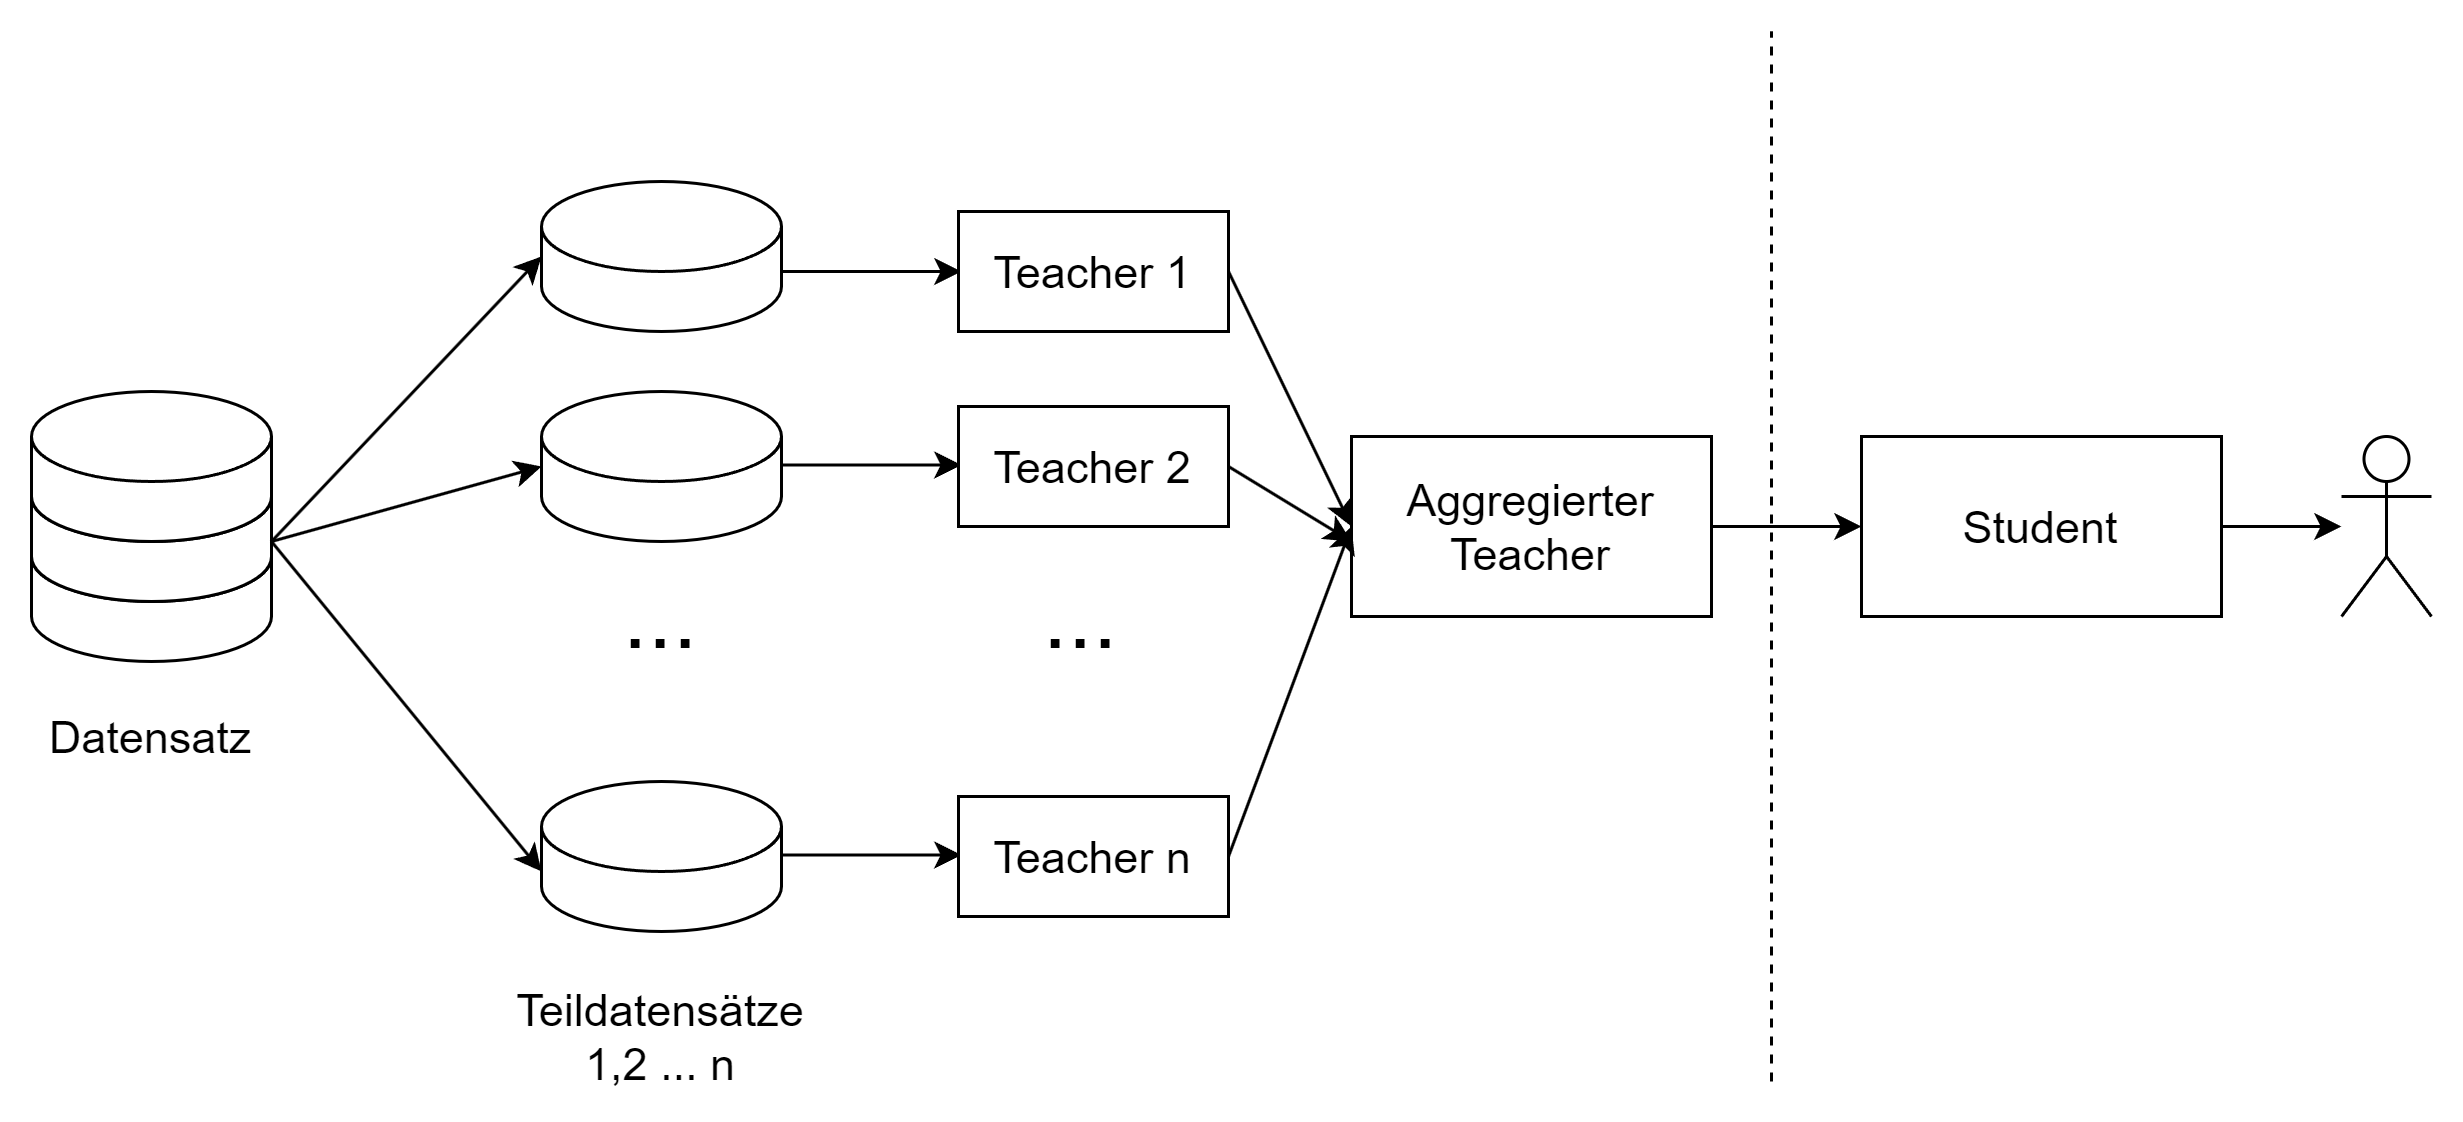
\includegraphics[width=15cm]{figures/pate_basic.png}
    \caption{PATE Architektur nach \cite{P-57}}
    \label{fig:pate_basic}
\end{figure} 

Abbildung \ref{fig:pate_basic} zeigt eine Übersicht der PATE Architektur.
Der Datensatz wird dabei zuerst in verschiedene Teildatensätze aufgeteilt. 
Für jeden dieser Teildatensätze wird anschließend ein sogenanntes Teacher oder Lehrer Modell trainiert.
Wenn das gesamte Modell eine Klassifikation aus 10 unterschiedlichen Klassen ist, dann muss jedes Teacher Modell ebenfalls diese Klassen abbilden.
Hierbei ist es ebenfalls wichtig, dass die Teildatensätze nicht zu klein sind, da ansonsten die Teacher Modelle nicht gut funktionieren würden.
Die Vorhersagen aller Teacher Modelle können aggregiert werden, indem die Vorhersagen der Teacher Modelle addiert werden. 
An dieser Stelle werden die Anzahlen jeder Klasse mittels des Laplace-Mechanismus verrauscht.
Diese Anzahlen können nun an das sogenannte Student oder Schüler Modell weitergegeben werden, welches die finale Vorhersage an den Nutzer weitergibt.
Die roten Pfeile der Abbildung zeigen dabei den Fluss einer Predction. 
Für den Nutzer ist nur der rechte Teil der gestrichelten Linie (Student Modell) erreichbar, der linke Teil nicht.

Theoretisch wäre es möglich, die Aggregation der Teacher Modelle direkt an den Nutzer zu geben.
Ein Student Modell könnte jedoch in die Hände eines Angreifers gelangen und wäre dennoch resistent gegen White Box Angriffe, wohingegen White Box Angriffe bei den Teacher Modellen problematischer wäre.
Zusätzlich bietet Student Modelle weitere Vorteile. So ist es beispielsweise möglich, die Teacher Modelle nur auf sensiblen Daten zu trainieren und nicht sensible (öffentliche) Daten mit in das Student Modell zu übergeben.